\documentclass[11pt]{article}   	% use "amsart" instead of "article" for AMSLaTeX format
\usepackage{geometry}                		% See geometry.pdf to learn the layout options. There are lots.
\geometry{a4paper}                   		% ... or a4paper or a5paper or ... 
%\geometry{landscape}                		% Activate for rotated page geometry
%\usepackage[parfill]{parskip}    		% Activate to begin paragraphs with an empty line rather than an indent
\usepackage{graphicx}				% Use pdf, png, jpg, or eps§ with pdflatex; use eps in DVI mode
								% TeX will automatically convert eps --> pdf in pdflatex		
\usepackage{amssymb}
\usepackage{caption}
\usepackage{subcaption}
\usepackage{subfig}

%SetFonts

%SetFonts


\title{Benchmarks for LBM}
\author{James Pritchard}
%\date{}							% Activate to display a given date or no date

\begin{document}
\maketitle
%\section{}
%\subsection{}

\begin{figure}
\centering
\begin{subfigure}{0.5\textwidth}
  \centering
  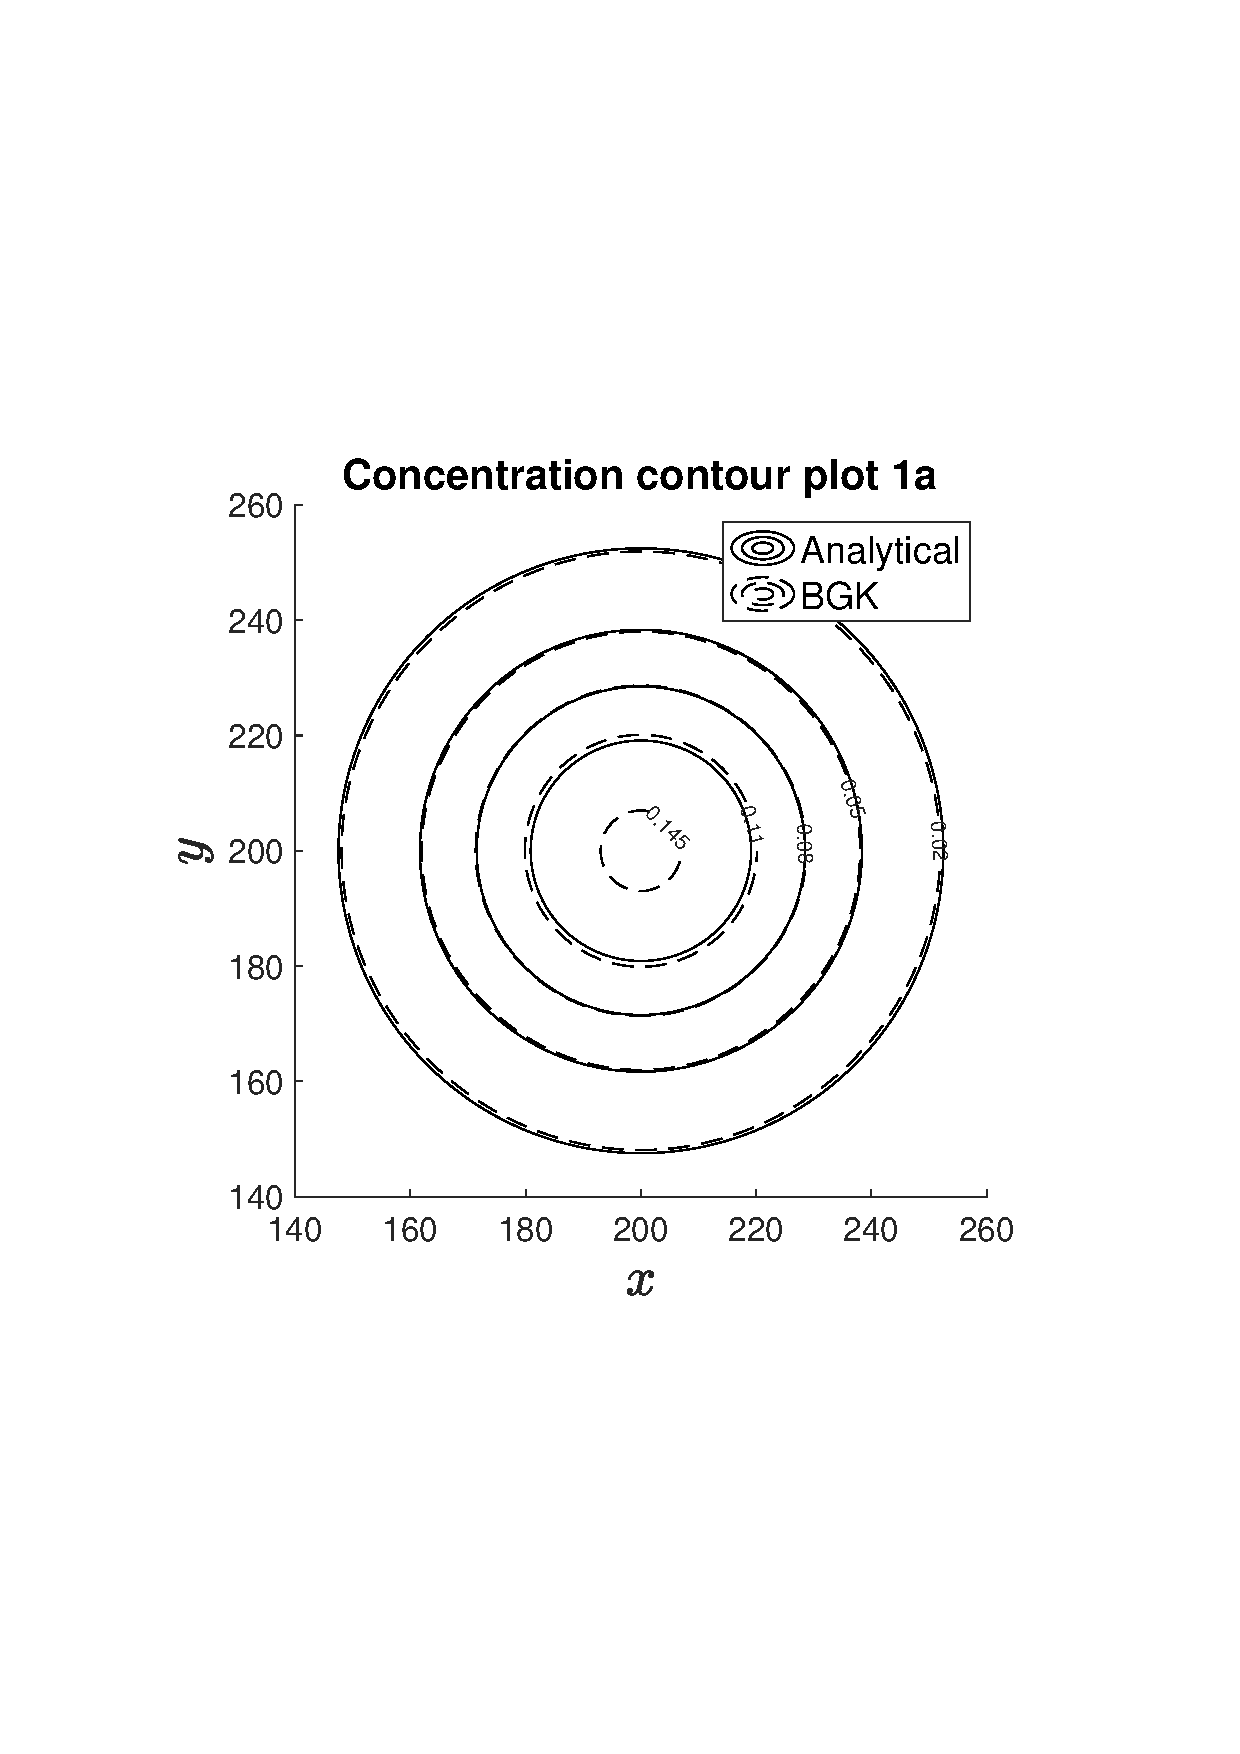
\includegraphics[width=1.2\linewidth]{concentration_contour_benchmark_1a}
  %\caption{A subfigure}
  %\label{fig:sub1}
\end{subfigure}%
\begin{subfigure}{0.5\textwidth}
  \centering
  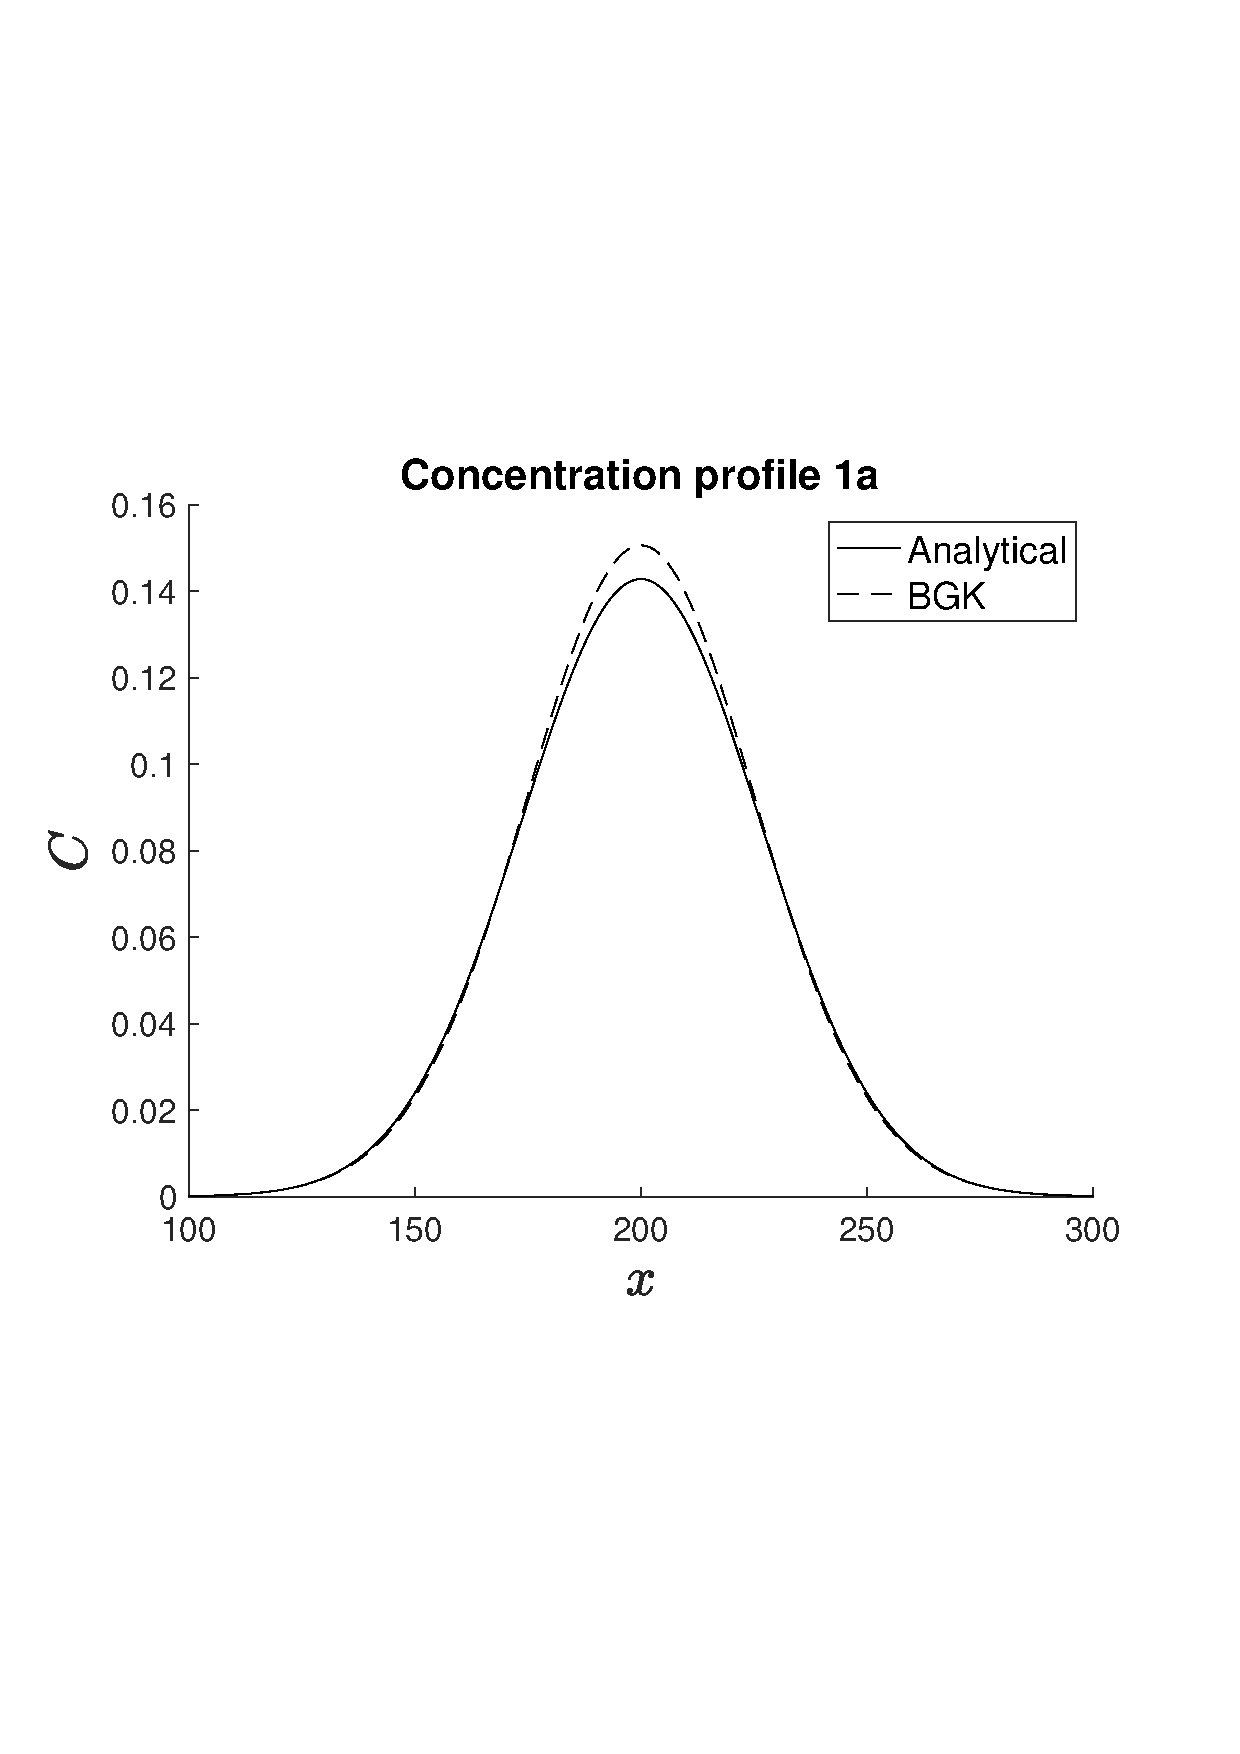
\includegraphics[width=1.2\linewidth]{concentration_profile_benchmark_1a}
  %\caption{A subfigure}
  %\label{fig:sub2}
\end{subfigure}
\caption{Concentration Contour and Profile for Benchmark 1a}
\label{fig:test}
\end{figure}

\begin{figure}
\centering
\begin{subfigure}{0.5\textwidth}
  \centering
  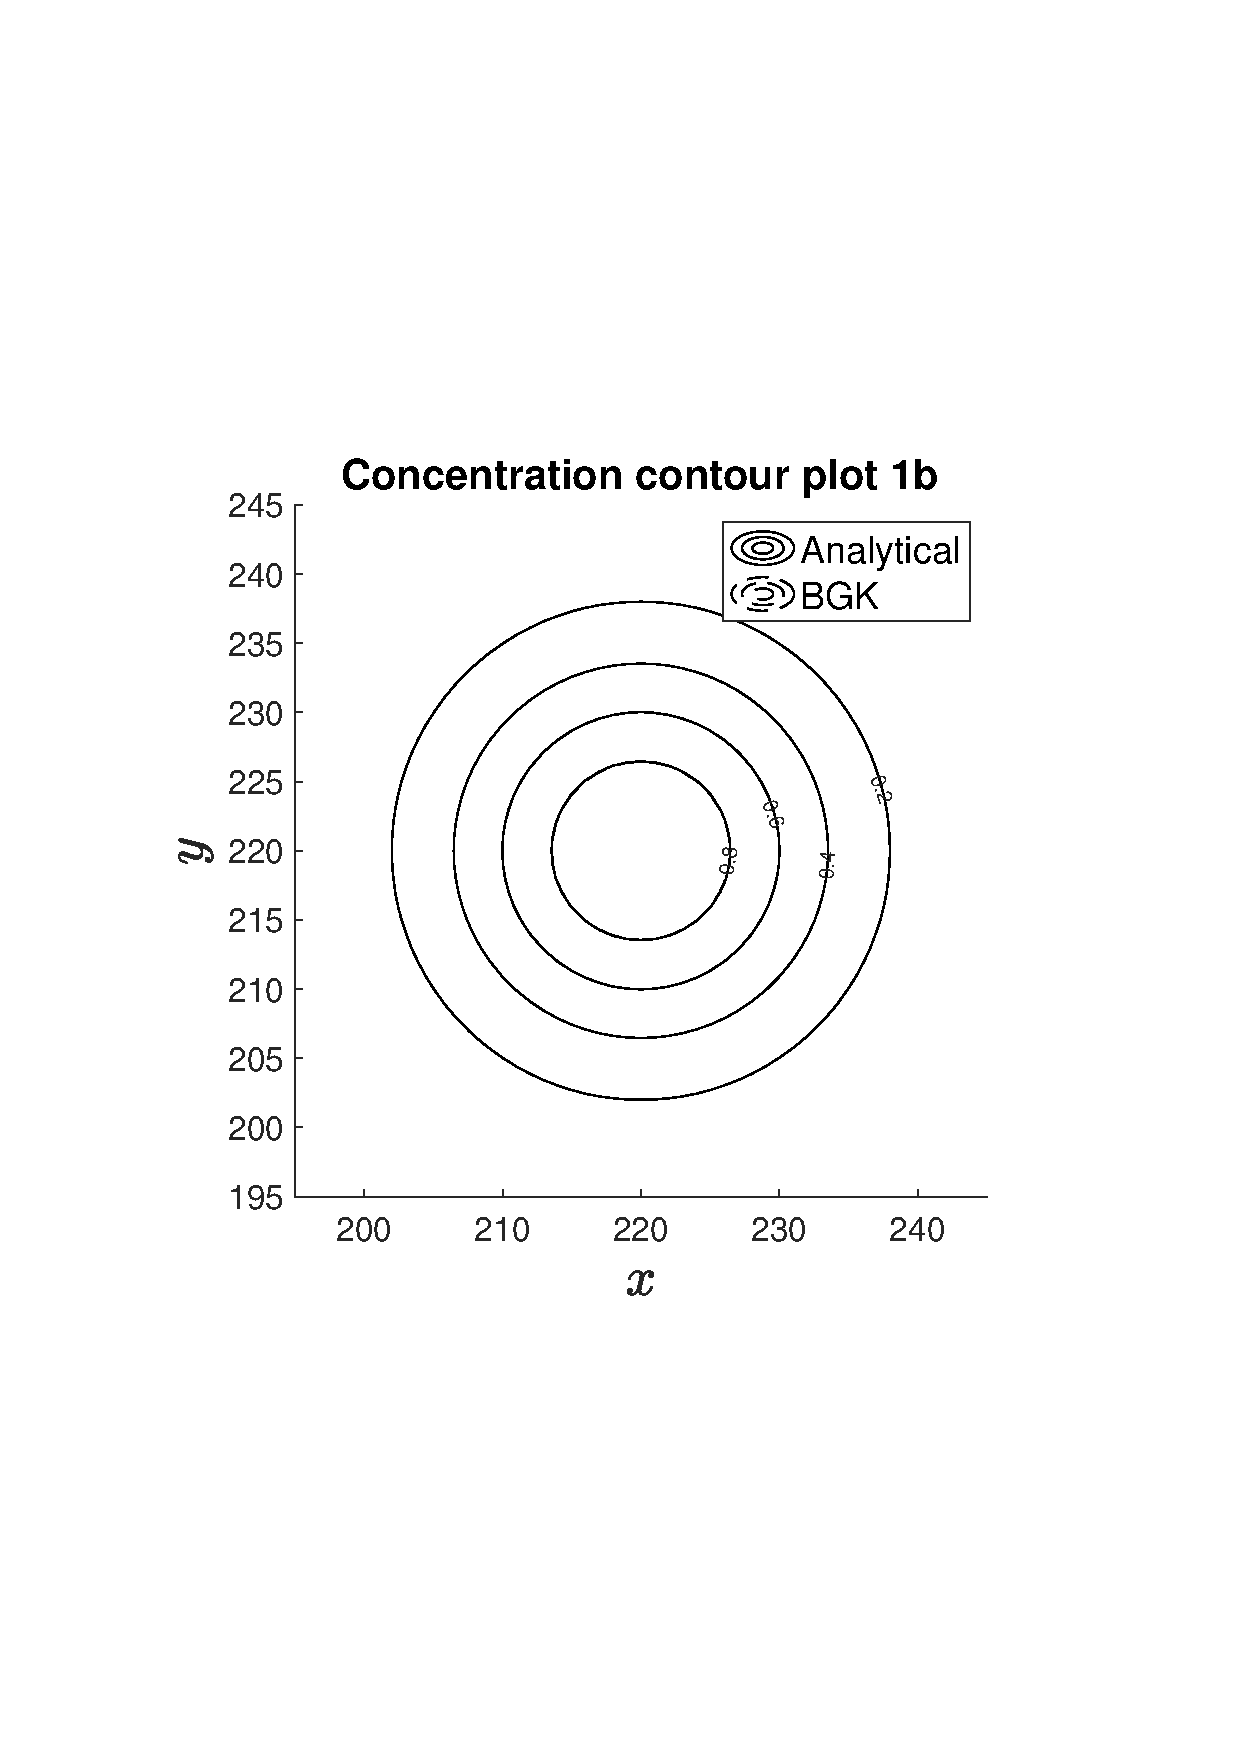
\includegraphics[width=1.2\linewidth]{concentration_contour_benchmark_1b}
  %\caption{A subfigure}
  %\label{fig:sub1}
\end{subfigure}%
\begin{subfigure}{0.5\textwidth}
  \centering
  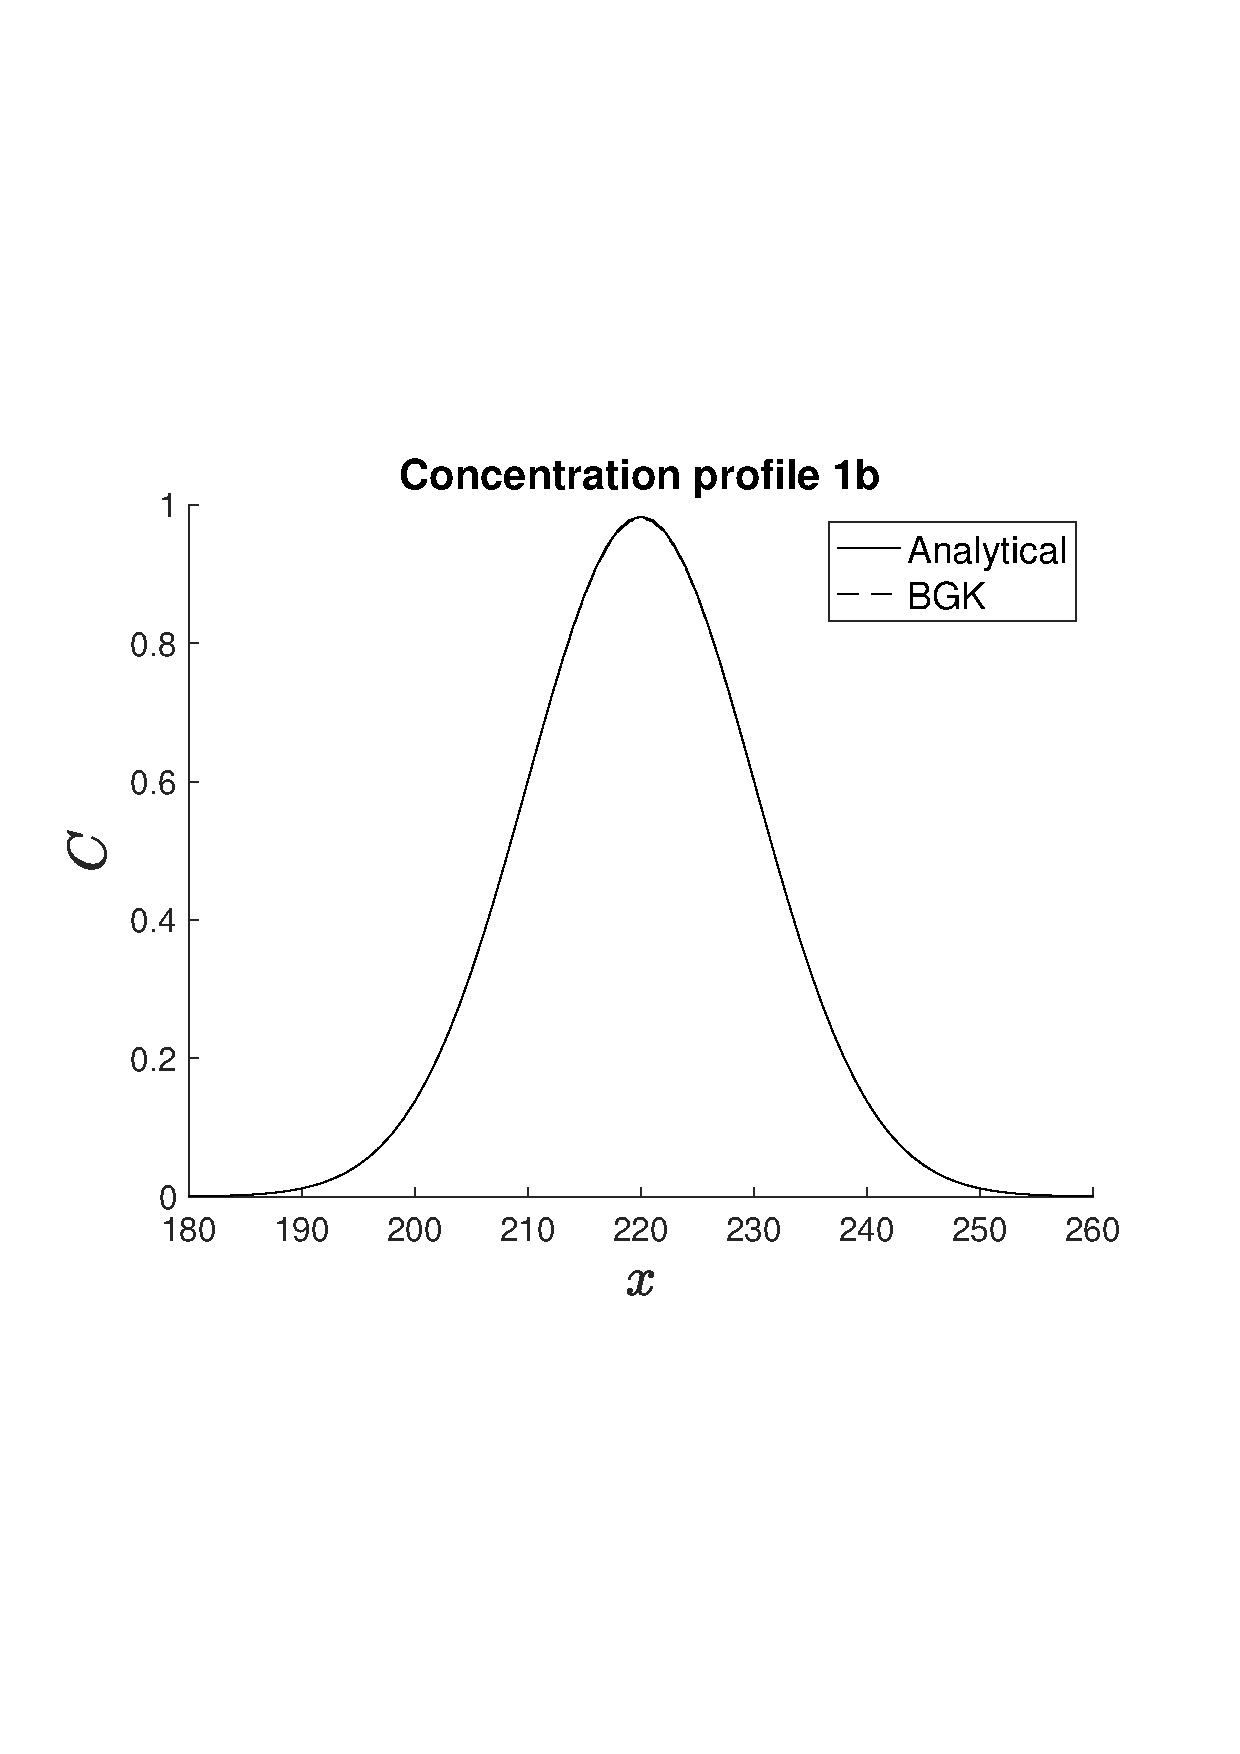
\includegraphics[width=1.2\linewidth]{concentration_profile_benchmark_1b}
  %\caption{A subfigure}
  %\label{fig:sub2}
\end{subfigure}
\caption{Concentration Contour and Profile for Benchmark 1b}
\label{fig:test}
\end{figure}




\end{document}  


















